\documentclass[10pt]{article}
\usepackage{titlesec}
\usepackage{geometry}
\geometry{verbose,tmargin=.9in,bmargin=.9in,lmargin=1.0in,rmargin=1.0in}
\usepackage{amsmath,amsfonts,amsthm,amssymb}
\usepackage{url}
\usepackage{color}
\usepackage[usenames,dvipsnames,svgnames,table]{xcolor}
\usepackage[colorlinks=true, linkcolor=red, urlcolor=blue, citecolor=gray]{hyperref}
\usepackage{float}
\usepackage{caption}
\usepackage{subcaption}
\usepackage{graphicx}
\usepackage{wrapfig}
\usepackage{booktabs}
\usepackage{longtable}
\usepackage{enumerate}
\usepackage{multicol}
\usepackage{etoolbox}
\newcommand{\bs}[1]{\boldsymbol{#1}}
\newcommand{\bv}[1]{\mathbf{#1}}
\usepackage{listings}

\definecolor{nyuDarkPurple}{HTML}{330662}
\definecolor{nyuOfficialPurple}{HTML}{57068c}

\newcommand{\spara}[1]{\vspace{.5em}\noindent {\large\sffamily\textcolor{nyuOfficialPurple}{#1}}}
\titleformat{\section}[hang]{\Large\sffamily\color{nyuDarkPurple}}{\thesection}{1em}{}
\titleformat{\subsection}[hang]{\large\sffamily\color{nyuDarkPurple}}{\thesection}{1em}{}
\titleformat{\subsubsection}[hang]{\normalsize\sffamily\color{gray}}{\thesection}{1em}{}

\usepackage{fancyhdr}
\pagestyle{fancy}
\lhead{
\includegraphics[width=4cm]{tandon_long_color.eps}}
\rhead{\thepage}
\pagenumbering{gobble}

\setcounter{secnumdepth}{0}

% math commands
\DeclareMathOperator{\R}{\mathbb{R}}
\newcommand{\E}{\mathbb{E}}

\begin{document}
	
\begin{center}
	\normalsize
	New York University Tandon School of Engineering
	
	Computer Science and Engineering
	\medskip
	
	\large
	CS-UY 4563: Written Homework 2. 
	
	Due Tuesday, February 18th, 2020, 11:59pm.
	\medskip
	
	\normalsize 
	\noindent \emph{Collaboration is allowed on this problem set, but solutions must be written-up individually. Please list the names of any collaborators at the top of your solution set, or write ``No Collaborators" if you worked alone.}
	\medskip
\end{center} 

\subsection{Problem 1: Practice Framing a Multiple Regression Problem (10pts)}
 An online retailer like Amazon wants to determine which products to promote based on reviews. They only want to promote products that are likely to sell. For each product, they have past sales as well as reviews. The reviews have both a numeric score (from 1 to 5) and text.
\begin{enumerate}[(a)]
	\item To formulate this as a machine learning problem, suggest a target variable that the online retailer could use.
	\item For the predictors of the target variable, a data scientist suggests to combine each review's numeric score with the frequency of occurrence of words that convey judgement like ``bad'', ``good'', ``broke'', or ``bargain''. The data scientist would like to use these features in a linear model.
	
	Describe one logical way to build feature vectors for each product. Think about normalization here!
	
	\item Suppose that some reviews have a numeric score from 1 to 5 and others have a score from 1 to 10. How would change your features?
	\item Now suppose the reviews have either:  a score from 1 to 5;  a rating that is simply good or bad; or no numeric rating at all. How would you change your features?
\end{enumerate}

\subsection{Problem 2: Thinking About Data Transformations (10pts)}
You are trying to fit a multiple linear regression model for a given data set. You have already transformed your data by appending a column of all ones, which resulted in a final data matrix:
\begin{align*}
X = \begin{bmatrix}
1 & x_{1,1} & x_{1,2} & \ldots & x_{1,d} \\
1 & x_{2,1} & x_{2,2} & \ldots & x_{2,d} \\
\vdots & \vdots & & \vdots\\
1 & x_{n,1} & x_{n,2} & \ldots & x_{n,d} \\
\end{bmatrix}
\end{align*}
However, your model does not seem to be working well. It obtains poor loss in both training and test. 
\begin{enumerate}[(a)]
	\item A friend suggests that you should try mean centering your data columns. In other words, for each $i$, compute the column mean $\bar{x}_i = \frac{1}{n}\sum_{j=1}^n x_{j,i}$ and subtract $\bar{x}_i$ from every entry in column $i$. Note that we won't mean center the first column, as doing so would set the 1s to 0s.
	Using Python broadcasting you might mean center by running:
	\begin{lstlisting}
	T = X[:,1:]
	X[:,1:] = T - np.mean(T,axis=0)
	\end{lstlisting}
	Do you expect your friend's suggestion to improve the performance of the linear model. Will it help in all cases? Some cases? No cases?
	
	\item Another friend suggests normalizing your data columns to have unit standard deviation. In other words for each $i$, compute the column standard deviation $\sigma_i = \sqrt{\frac{1}{n}\sum_{j=1}^n (x_{i,j} - \bar{x}_i)^2}$ and \emph{divide} every column by $\sigma_i$. 
	Using Python broadcasting you might run:
	\begin{lstlisting}
	T = X[:,1:]
	X[:,1:] = T/np.std(T,axis=0)
	\end{lstlisting}
	Do you expect your friends suggestion to improve the performance of the linear model. Will it help in all cases? Some cases? No cases?
	
	\item Would your answers to either of the two questions above change if you were fitting the model with $\ell_2$ regularization? In other words, instead of minimizing the squared loss $L(\bs{\beta}) = \|\bv{y} - \bv{X}\bs{\beta}\|_2^2$ alone, you were minimizing $L(\bs{\beta}) + \lambda\|\bs{\beta}\|_2^2$. 

\end{enumerate}


\subsection{Problem 3: Practice With Gradients (10pts)}
For $\bv{X} \in \R^{n\times d}$ and target vector $\bv{y} \in \R^n$, consider fitting a linear model of the form:
\begin{align*}
f_{\bs{\beta}}(\bv{x}) = \bv{X}\bs{\beta}
\end{align*}
under the so-called $\ell_p$ loss: $L_p(\bs{\beta}) = \|\bv{y} - f_{\bs{\beta}}(\bv{x})\|_p^p$. Here $\|\cdot \|_p^p$ denotes the $\ell_p$ norm raised to the $p$ power. I.e. for any even integer $p = 2,4,6, \ldots$
\begin{align*}
\|\bv{z}\|_p^p = \sum_{i=1}^n z_i^p
\end{align*}

\begin{enumerate}[(a)]
	\item Derive an expression for $\nabla g(\bv{z})$ where $g(\bv{z}) = \|\bv{z}\|_p^p$. 
	
	\item Derive an expression for $\nabla L_p(\bs{\beta})$. \textbf{Hint:} Use chain rule.
\end{enumerate}

\subsection{Problem 4: Piecewise Linear Regression via Feature Transformations (15pts)}
Your goal is to fit a \emph{piecewise} linear model to a single variate dataset of the form $(x_1, y_1), \ldots, (x_n, y_n)$ where all values are scalars. We will only use two pieces. In other words, for some known value $\lambda$, 
\begin{align*}
f(x_i) = \begin{cases}
a_1 + s_1x_i & \text{ for $x_i < \lambda$}\\ 
a_2 + s_2x_i & \text{ for $x_i \geq \lambda$}
\end{cases}
\end{align*}
with the additional \textbf{constraint} that $a_1 + s_1\lambda = a_2 + s_2\lambda$. This constraint ensures that our two linear models actually ``meet'' at $x = \lambda$, which means we get a continuous prediction function.

For example, when $\lambda = 100$, a piecewise linear fit for our MPG data might look like:
\begin{figure}[H]
	\centering
	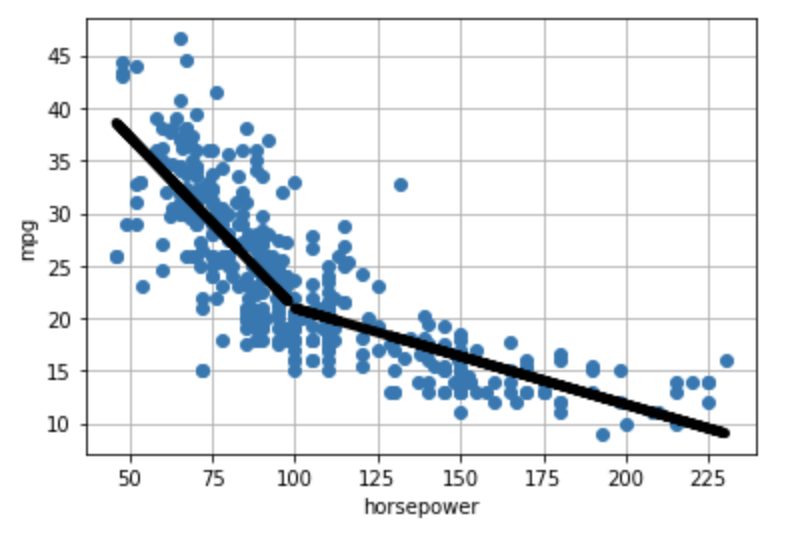
\includegraphics[width=.4\textwidth]{piecewise_fit.png} 
\end{figure}

\begin{enumerate}[(a)]
	\item Show that this model is equivalent to the following \textbf{unconstrained} model:
	\begin{align*}
	f(x_i) = \begin{cases}
		a_1 + s_1x_i & \text{ for $x_i < \lambda$}\\ 
		a_1 + s_1 \lambda - s_2 \lambda + s_2x_i & \text{ for $x_i \geq \lambda$}
	\end{cases}
	\end{align*}
	
	\item Show how to fit an optimal $f$ under the squared loss using an algorithm for multiple linear regression. In particular, your approach should:
	\begin{itemize}
		\item Transform the input data to form a data matrix $\bv{X}$ with multiple columns.
		\item Use a multiple regression algorithm to find the $\bs{\beta}$ which minimizes $\|\bv{y} - \bv{X}\bs{\beta}\|_2^2.$
		\item Extract from the optimal $\bs{\beta}$ optimal values for $a_1, s_1, s_2$. 
	\end{itemize} 
	You need to describe 1) a correct data transformation and 2) a correct mapping from $\bs{\beta}$ to $a_1, s_1, s_2$. 
	\textbf{Note that in our model $\lambda$ is known. It is not a model parameter which needs to be optimized.}
	
	\item Implement your algorithm in Python and apply it to the dataset from \texttt{demo\_auto\_mpg.ipynb}. Produce a piecewise linear fit for MPG as a function of Horsepower using the value $\lambda = 100$. Plot the result. You can attach a Jupyter notebook to your submission, or simply include the printed code and plot. 
	
	\item (\textbf{5pts bonus}) Modify your approach to handle the case when $\lambda$ is unknown. Again obtain a fit for MPG vs. horsepower. What value of $\lambda$ gives the optimal fit? Include any modified code and a plot of your result.
\end{enumerate}






\end{document}